\section{Capítulo 9 -- Algoritmos gulosos e programação dinâmica}

Muitos problemas pedem não uma resposta qualquer, mas a \textbf{melhor} resposta: o troco com menos moedas, o maior número de reuniões em uma sala, a rede de estradas mais barata, a mochila com o maior valor. Esses são os \textbf{problemas de otimização}. Testar todas as possibilidades quase sempre é inviável, porque elas crescem de forma exponencial. Neste capítulo você vai conhecer duas técnicas para resolvê-los de forma eficiente: os \textbf{algoritmos gulosos}, que tomam a melhor decisão do momento e nunca voltam atrás, e a \textbf{programação dinâmica}, que resolve cada subproblema uma única vez e guarda a resposta. No caminho, você vai ver o algoritmo de Kruskal, prometido no Capítulo 6.

\subsection{9.1 Algoritmos gulosos}

Um algoritmo \textbf{guloso} constrói a solução passo a passo e, a cada passo, faz a escolha que parece melhor \textbf{naquele momento}, sem pensar nas consequências e sem desfazer escolhas anteriores. Você já conhece três: o Dijkstra, que sempre trata o vértice mais próximo; o Prim, que sempre pega a aresta mais barata; e a ordenação por seleção, que sempre busca o menor elemento.

O exemplo mais familiar é o troco. Para dar 87 centavos com as moedas brasileiras (1 real, 50, 25, 10, 5 e 1 centavo), qualquer caixa faz assim: usa a maior moeda que ainda cabe, desconta, e repete. São 50 + 25 + 10 + 1 + 1, cinco moedas, e não há como usar menos.

\begin{codigo}
\begin{Verbatim}[breaklines=true, breaksymbolleft={}, fontsize=\footnotesize]
#include <vector>

// usa sempre a maior moeda que ainda cabe
// (as moedas precisam estar em ordem decrescente)
vector<int> trocoGuloso(const vector<int> &moedas, int valor) {
    vector<int> usadas;
    for (int m : moedas) {
        while (valor >= m) {
            usadas.push_back(m);
            valor -= m;
        }
    }
    return usadas;
}

void mostrar(const vector<int> &v) {
    for (int x : v) cout << x << " ";
    cout << endl;
}

int main() {
    mostrar(trocoGuloso({100, 50, 25, 10, 5, 1}, 87));
    // 50 25 10 1 1
    mostrar(trocoGuloso({4, 3, 1}, 6));   // 4 1 1
}
\end{Verbatim}
\end{codigo}

A segunda chamada mostra o perigo. Com moedas de 4, 3 e 1, o guloso dá 6 como $4 + 1 + 1$, três moedas, mas $3 + 3$ usa só duas. A primeira escolha, a moeda de 4, parecia a melhor e estragou o resto. Com as moedas brasileiras o guloso sempre acerta, mas isso é uma propriedade daquele conjunto de moedas, e não do algoritmo.

Um algoritmo guloso só dá a resposta ótima quando o problema tem duas propriedades:

\begin{itemize}
  \item \textbf{Escolha gulosa}: existe uma solução ótima que começa pela escolha gulosa. Ou seja, fazer a escolha que parece melhor agora nunca impede de chegar ao melhor resultado.
  \item \textbf{Subestrutura ótima}: depois da escolha, o que sobra é um problema menor do mesmo tipo, e a solução ótima do todo contém a solução ótima dessa parte.
\end{itemize}

Quando as duas valem, o guloso costuma ser o algoritmo mais simples e mais rápido possível. Quando não valem, ele dá uma resposta que pode estar longe da melhor, sem nenhum aviso. Por isso, todo algoritmo guloso precisa de um argumento de que a escolha é segura, ou de um contraexemplo que mostre que não é.

\subsection{9.2 Seleção de atividades}

Um auditório recebe pedidos para várias palestras, cada uma com horário de início e de término, e duas palestras não podem acontecer ao mesmo tempo. Qual é o \textbf{maior número} de palestras que cabem na agenda?

Há várias escolhas gulosas possíveis, e a maioria falha. Escolher a que \textbf{começa primeiro} falha se ela durar o dia inteiro: uma única palestra ocupa o auditório. Escolher a \textbf{mais curta} falha se ela estiver bem no meio de outras duas que caberiam juntas. A escolha certa é a palestra que \textbf{termina primeiro}: ela deixa o auditório livre o mais cedo possível, sobrando o máximo de tempo para as outras.

\begin{center}
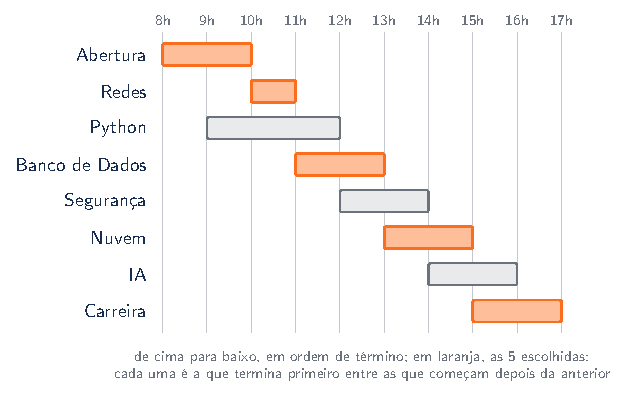
\includegraphics[width=0.85\linewidth,keepaspectratio]{imagens/capitulo-09_atividades.pdf}
\end{center}

Por que essa escolha é segura? Pegue qualquer agenda ótima. Se a primeira palestra dela não for a que termina primeiro, troque-a por esta: como ela termina mais cedo, não pode se sobrepor às seguintes, e a agenda continua com o mesmo número de palestras. Esse argumento de troca é a forma típica de provar que um guloso está correto.

\begin{codigo}
\begin{Verbatim}[breaklines=true, breaksymbolleft={}, fontsize=\footnotesize]
#include <vector>
#include <algorithm>   // sort

struct Palestra {
    string nome;
    int inicio, fim;   // horas
};

// recebe uma cópia: a lista original não é reordenada
vector<Palestra> escolher(vector<Palestra> palestras) {
    sort(palestras.begin(), palestras.end(),
         [](const Palestra &a, const Palestra &b) {
             return a.fim < b.fim;  // termina primeiro
         });
    vector<Palestra> escolhidas;
    int livreDesde = 0;         // fim da última escolhida
    for (const Palestra &p : palestras) {
        if (p.inicio >= livreDesde) {   // não se sobrepõe
            escolhidas.push_back(p);
            livreDesde = p.fim;
        }
    }
    return escolhidas;
}

int main() {
    vector<Palestra> agenda = {
        {"Abertura", 8, 10}, {"Python", 9, 12}, {"Redes", 10, 11},
        {"Banco de Dados", 11, 13}, {"Segurança", 12, 14},
        {"Nuvem", 13, 15}, {"IA", 14, 16}, {"Carreira", 15, 17}};
    for (const Palestra &p : escolher(agenda)) {
        cout << p.nome << " (" << p.inicio << "h-"
             << p.fim << "h)" << endl;
    }
    // Abertura (8h-10h), Redes (10h-11h),
    // Banco de Dados (11h-13h), Nuvem (13h-15h),
    // Carreira (15h-17h)
}
\end{Verbatim}
\end{codigo}

O critério de ordenação é a mesma função anônima (\textit{lambda}) usada no Capítulo 8. Depois da ordenação, que custa $O(n \log n)$, uma única passada escolhe as palestras em $O(n)$. O algoritmo inteiro é $O(n \log n)$.

\subsection{9.3 Árvore geradora mínima: algoritmo de Kruskal}

No Capítulo 6, o Prim construiu a árvore geradora mínima a partir de um vértice, fazendo a árvore crescer aresta por aresta. O \textbf{algoritmo de Kruskal} é outra estratégia gulosa para o mesmo problema, ainda mais direta:

\begin{enumerate}
  \item Ordene todas as arestas da mais leve para a mais pesada.
  \item Percorra as arestas nessa ordem. Aceite cada uma que ligue dois vértices que ainda \textbf{não estão conectados}; recuse as que fechariam um ciclo.
  \item Pare quando tiver $V - 1$ arestas.
\end{enumerate}

\begin{center}
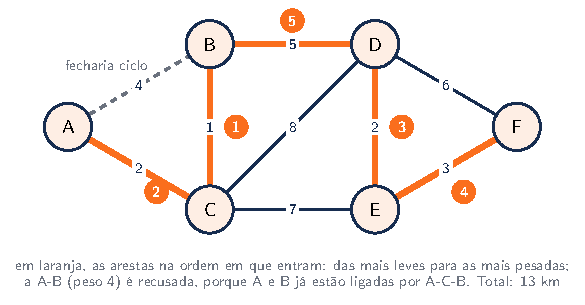
\includegraphics[width=0.8\linewidth,keepaspectratio]{imagens/capitulo-09_kruskal.pdf}
\end{center}

No grafo das cidades, o Kruskal escolhe exatamente as mesmas cinco estradas que o Prim, com o mesmo total de 13 km, mas em outra ordem: o Prim mantém uma única árvore que cresce, enquanto o Kruskal junta vários pedaços soltos que vão se unindo.

\begin{center}
\begin{tabular}{@{}p{0.16\linewidth}p{0.1\linewidth}p{0.64\linewidth}@{}}
\toprule
\rowcolor{headergray}
\tblheader{Aresta} & \tblheader{Peso} & \tblheader{Decisão} \\
\midrule
B-C & 1 & aceita: grupos \{A\} \{B, C\} \{D\} \{E\} \{F\} \\
\rowcolor{rowgray} A-C & 2 & aceita: \{A, B, C\} \{D\} \{E\} \{F\} \\
D-E & 2 & aceita: \{A, B, C\} \{D, E\} \{F\} \\
\rowcolor{rowgray} E-F & 3 & aceita: \{A, B, C\} \{D, E, F\} \\
A-B & 4 & recusada: A e B já estão no mesmo grupo \\
\rowcolor{rowgray} B-D & 5 & aceita: \{A, B, C, D, E, F\}; são 5 arestas, fim \\
\bottomrule
\end{tabular}
\end{center}

\subsubsection{Conjuntos disjuntos (\textit{union-find})}

A pergunta que o Kruskal faz a cada aresta é: ``estes dois vértices já estão no mesmo grupo?''. Percorrer o grafo para responder custaria caro. A estrutura certa é a de \textbf{conjuntos disjuntos} (\textit{union-find}), que guarda grupos que não se misturam e oferece duas operações:

\begin{itemize}
  \item \texttt{raiz(x)}: devolve o representante do grupo de \texttt{x}. Dois elementos estão no mesmo grupo se tiverem a mesma raiz.
  \item \texttt{unir(a, b)}: junta os grupos de \texttt{a} e \texttt{b} em um só.
\end{itemize}

Cada grupo é uma árvore guardada em um vetor \texttt{pai}, como o heap do Capítulo 8: \texttt{pai[x]} é o pai de \texttt{x}, e a raiz é quem é pai de si mesmo. Unir dois grupos é só pendurar a raiz de um embaixo da raiz do outro.

\begin{codigo}
\begin{Verbatim}[breaklines=true, breaksymbolleft={}, fontsize=\footnotesize]
// trecho
class ConjuntosDisjuntos {
private:
    vector<int> pai, tamanho;

public:
    explicit ConjuntosDisjuntos(int n) : pai(n), tamanho(n, 1) {
        for (int i = 0; i < n; i++) pai[i] = i;  // sozinhos
    }

    int raiz(int x) {
        while (pai[x] != x) {
            pai[x] = pai[pai[x]];   // pula para o avô
            x = pai[x];
        }
        return x;
    }

    bool unir(int a, int b) {       // false se já estavam juntos
        a = raiz(a);
        b = raiz(b);
        if (a == b) return false;
        if (tamanho[a] < tamanho[b]) swap(a, b);
        pai[b] = a;                 // menor embaixo do maior
        tamanho[a] += tamanho[b];
        return true;
    }
};
\end{Verbatim}
\end{codigo}

Dois truques mantêm as árvores baixas. Na união, o grupo \textbf{menor} é pendurado no maior, para a altura crescer o mínimo possível. E, a cada \texttt{raiz}, a linha \texttt{pai[x] = pai[pai[x]]} faz cada nó do caminho pular para o avô, encurtando o caminho para as próximas consultas. Com os dois juntos, cada operação custa, na prática, tempo constante.

\begin{codigo}
\begin{Verbatim}[breaklines=true, breaksymbolleft={}, fontsize=\footnotesize]
#include <vector>
#include <tuple>
#include <algorithm>   // sort
#include <utility>     // swap

class ConjuntosDisjuntos {
private:
    vector<int> pai, tamanho;

public:
    explicit ConjuntosDisjuntos(int n) : pai(n), tamanho(n, 1) {
        for (int i = 0; i < n; i++) pai[i] = i;  // sozinhos
    }

    int raiz(int x) {
        while (pai[x] != x) {
            pai[x] = pai[pai[x]];   // pula para o avô
            x = pai[x];
        }
        return x;
    }

    bool unir(int a, int b) {       // false se já estavam juntos
        a = raiz(a);
        b = raiz(b);
        if (a == b) return false;
        if (tamanho[a] < tamanho[b]) swap(a, b);
        pai[b] = a;                 // menor embaixo do maior
        tamanho[a] += tamanho[b];
        return true;
    }
};

using Ligacao = tuple<int, int, int>;   // (peso, de, para)

int kruskal(int n, vector<Ligacao> arestas,
            vector<Ligacao> &escolhidas) {
    sort(arestas.begin(), arestas.end());   // pelo peso primeiro
    ConjuntosDisjuntos grupos(n);
    int total = 0;
    for (const auto &[peso, de, para] : arestas) {
        if (grupos.unir(de, para)) {        // não fecha ciclo
            escolhidas.push_back({peso, de, para});
            total += peso;
            int usadas = static_cast<int>(escolhidas.size());
            if (usadas == n - 1) break;       // árvore completa
        }
    }
    return total;
}

int main() {
    const string NOMES = "ABCDEF";
    enum { A, B, C, D, E, F };
    vector<Ligacao> estradas = {
        {4, A, B}, {2, A, C}, {1, B, C}, {5, B, D}, {8, C, D},
        {7, C, E}, {2, D, E}, {6, D, F}, {3, E, F}};
    vector<Ligacao> escolhidas;
    int total = kruskal(6, estradas, escolhidas);
    for (const auto &[peso, de, para] : escolhidas) {
        cout << NOMES[de] << "-" << NOMES[para] << " ";
    }
    cout << endl;                           // B-C A-C D-E E-F B-D
    cout << "Total: " << total << " km" << endl;   // Total: 13 km
}
\end{Verbatim}
\end{codigo}

Como cada aresta é uma tupla (peso, de, para) e as tuplas são comparadas campo a campo, a \texttt{sort} ordena pelo peso sem precisar de critério próprio. O custo do Kruskal é dominado por essa ordenação: $O(E \log E)$. Ele costuma ser preferido ao Prim quando o grafo já vem como uma lista de arestas, e o Prim, quando vem como lista de adjacência.

\subsection{9.4 Programação dinâmica}

Quando a escolha gulosa não é segura, como no troco com moedas de 4, 3 e 1, é preciso considerar todas as opções. A recursão faz isso naturalmente, mas costuma recalcular a mesma coisa muitas vezes. O exemplo clássico é a sequência de Fibonacci, em que cada termo é a soma dos dois anteriores: 0, 1, 1, 2, 3, 5, 8, 13\ldots{}

\begin{center}
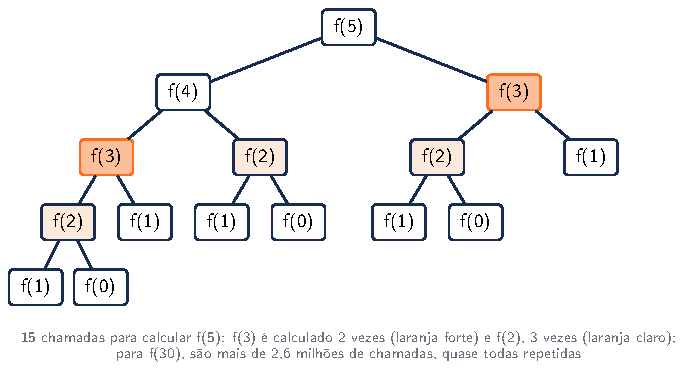
\includegraphics[width=0.9\linewidth,keepaspectratio]{imagens/capitulo-09_fibonacci.pdf}
\end{center}

A recursão direta, \texttt{fib(n) = fib(n - 1) + fib(n - 2)}, abre duas chamadas por nível, e o número de chamadas cresce como $1{,}6^n$. Mas só existem $n + 1$ subproblemas diferentes: \texttt{fib(0)} até \texttt{fib(n)}. Todo o resto é repetição.

A \textbf{programação dinâmica} resolve cada subproblema \textbf{uma única vez} e guarda a resposta em uma tabela. Ela se aplica quando o problema tem \textbf{subestrutura ótima}, como no guloso, e \textbf{subproblemas sobrepostos}: os mesmos subproblemas aparecem muitas vezes. Há dois jeitos de fazer isso:

\begin{itemize}
  \item \textbf{Memorização} (\textit{memoization}, de cima para baixo): mantenha a recursão, mas antes de calcular, veja se a resposta já está guardada; depois de calcular, guarde.
  \item \textbf{Tabulação} (de baixo para cima): preencha a tabela em um laço, dos casos menores para os maiores, de modo que cada posição só dependa de posições já preenchidas.
\end{itemize}

\begin{codigo}
\begin{Verbatim}[breaklines=true, breaksymbolleft={}, fontsize=\footnotesize]
#include <vector>

long long chamadas = 0;

long long fibIngenuo(int n) {
    chamadas++;
    if (n < 2) return n;
    return fibIngenuo(n - 1) + fibIngenuo(n - 2);
}

// memorização: memo[n] == -1 significa "ainda não calculado"
long long fibMemo(int n, vector<long long> &memo) {
    if (n < 2) return n;
    if (memo[n] != -1) return memo[n];       // já sabemos
    memo[n] = fibMemo(n - 1, memo) + fibMemo(n - 2, memo);
    return memo[n];
}

// tabulação: preenche de baixo para cima
long long fibTabela(int n) {
    if (n < 2) return n;
    vector<long long> f(n + 1);
    f[0] = 0;
    f[1] = 1;
    for (int i = 2; i <= n; i++) f[i] = f[i - 1] + f[i - 2];
    return f[n];
}

int main() {
    cout << fibIngenuo(30) << " em " << chamadas
         << " chamadas" << endl;     // 832040 em 2692537 chamadas
    vector<long long> memo(91, -1);
    cout << fibMemo(90, memo) << endl;   // 2880067194370816120
    cout << fibTabela(90) << endl;       // 2880067194370816120
}
\end{Verbatim}
\end{codigo}

As duas versões com tabela fazem $O(n)$ somas. A diferença é brutal: a versão ingênua leva mais de 2,6 milhões de chamadas para \texttt{fib(30)}, e para \texttt{fib(90)} precisaria de cerca de $9 \times 10^{18}$ chamadas, quase 300 anos a um bilhão de chamadas por segundo; as outras calculam \texttt{fib(90)} instantaneamente. Na tabulação, como cada termo só depende dos dois anteriores, dá até para trocar o vetor por duas variáveis e usar memória $O(1)$.

Para resolver um problema com programação dinâmica, siga sempre os mesmos passos:

\begin{enumerate}
  \item \textbf{Defina o subproblema} em palavras: ``\texttt{menor[v]} é o menor número de moedas para formar o valor \texttt{v}''.
  \item \textbf{Escreva a recorrência}: como a resposta de um subproblema se calcula a partir de subproblemas menores.
  \item \textbf{Defina os casos base}: os subproblemas que se resolvem sem recorrência.
  \item \textbf{Escolha a ordem de cálculo}: cada posição da tabela só pode usar posições já calculadas.
  \item \textbf{Reconstrua a solução}, se o problema pedir a escolha e não só o valor: guarde qual opção gerou cada resposta.
\end{enumerate}

\subsection{9.5 Troco com o menor número de moedas}

Voltando ao troco: seja \texttt{menor[v]} o menor número de moedas que somam \texttt{v}. A última moeda usada é alguma moeda \texttt{m}, e o que vem antes dela é um troco ótimo para \texttt{v - m}. Como não sabemos qual é \texttt{m}, testamos todas:

\begin{center}
\texttt{menor[v] = 1 + min(menor[v - m])}, para cada moeda \texttt{m <= v}, \\
com o caso base \texttt{menor[0] = 0}.
\end{center}

Com moedas de 1, 3 e 4, a tabela fica assim. A linha ``última moeda'' guarda a moeda que deu o mínimo, e serve para reconstruir o troco: para 6, a última é 3; para $6 - 3 = 3$, a última também é 3. O troco é $3 + 3$.

\begin{center}
\begin{tabular}{@{}p{0.22\linewidth}p{0.06\linewidth}p{0.06\linewidth}p{0.06\linewidth}p{0.06\linewidth}p{0.06\linewidth}p{0.06\linewidth}p{0.06\linewidth}@{}}
\toprule
\rowcolor{headergray}
\tblheader{valor} & \tblheader{0} & \tblheader{1} & \tblheader{2} & \tblheader{3} & \tblheader{4} & \tblheader{5} & \tblheader{6} \\
\midrule
menor & 0 & 1 & 2 & 1 & 1 & 2 & 2 \\
\rowcolor{rowgray} última moeda & -- & 1 & 1 & 3 & 4 & 1 & 3 \\
\bottomrule
\end{tabular}
\end{center}

\begin{codigo}
\begin{Verbatim}[breaklines=true, breaksymbolleft={}, fontsize=\footnotesize]
#include <vector>

vector<int> trocoMinimo(const vector<int> &moedas, int valor) {
    const int INF = valor + 1;          // mais que o possível
    vector<int> menor(valor + 1, INF), ultima(valor + 1, 0);
    menor[0] = 0;                       // caso base
    for (int v = 1; v <= valor; v++) {  // do menor ao maior
        for (int m : moedas) {
            if (m <= v && menor[v - m] + 1 < menor[v]) {
                menor[v] = menor[v - m] + 1;
                ultima[v] = m;          // para reconstruir
            }
        }
    }
    vector<int> usadas;
    if (menor[valor] == INF) return usadas;   // impossível
    for (int v = valor; v > 0; v -= ultima[v]) {
        usadas.push_back(ultima[v]);
    }
    return usadas;
}

void mostrar(const vector<int> &v) {
    for (int x : v) cout << x << " ";
    cout << endl;
}

int main() {
    mostrar(trocoMinimo({1, 3, 4}, 6));     // 3 3
    mostrar(trocoMinimo({1, 5, 10, 25, 50, 100}, 87));
    // 1 1 10 25 50: as mesmas 5 moedas do guloso
    cout << trocoMinimo({5, 10}, 7).size() << endl;   // 0
}
\end{Verbatim}
\end{codigo}

A programação dinâmica acerta para qualquer conjunto de moedas e também descobre quando o troco é impossível, como 7 centavos só com moedas de 5 e 10. O preço é o custo: $O(\text{valor} \times \text{número de moedas})$, contra o $O(\text{número de moedas usadas})$ do guloso.

\subsection{9.6 O problema da mochila}

Uma pessoa vai acampar com uma mochila que aguenta 7 kg e precisa escolher o que levar. Cada item tem um peso e um valor (a utilidade dele na viagem), e cada um é levado inteiro ou deixado em casa. Qual combinação dá o maior valor sem passar do peso? É o \textbf{problema da mochila 0/1}.

\begin{center}
\begin{tabular}{@{}p{0.3\linewidth}p{0.14\linewidth}p{0.14\linewidth}p{0.26\linewidth}@{}}
\toprule
\rowcolor{headergray}
\tblheader{Item} & \tblheader{Peso} & \tblheader{Valor} & \tblheader{Valor por kg} \\
\midrule
lanterna & 1 kg & 1 & 1,00 \\
\rowcolor{rowgray} cantil & 3 kg & 4 & 1,33 \\
saco de dormir & 4 kg & 5 & 1,25 \\
\rowcolor{rowgray} barraca & 5 kg & 7 & 1,40 \\
\bottomrule
\end{tabular}
\end{center}

A ideia gulosa seria levar primeiro o item com mais valor por quilo: a barraca (5 kg). Depois, só a lanterna cabe, e o total é 8. Mas o cantil com o saco de dormir pesam exatamente 7 kg e valem 9. O guloso falha.

Na programação dinâmica, o subproblema é \texttt{melhor[i][c]}: o maior valor possível usando só os \texttt{i} primeiros itens com uma mochila de capacidade \texttt{c}. Para o item \texttt{i}, só há duas opções: deixá-lo, e a resposta é \texttt{melhor[i - 1][c]}; ou levá-lo, se couber, e a resposta é o valor dele mais \texttt{melhor[i - 1][c - peso]}. A resposta é a maior das duas.

\begin{center}
\begin{tabular}{@{}p{0.27\linewidth}p{0.05\linewidth}p{0.05\linewidth}p{0.05\linewidth}p{0.05\linewidth}p{0.05\linewidth}p{0.05\linewidth}p{0.05\linewidth}p{0.05\linewidth}@{}}
\toprule
\rowcolor{headergray}
\tblheader{capacidade} & \tblheader{0} & \tblheader{1} & \tblheader{2} & \tblheader{3} & \tblheader{4} & \tblheader{5} & \tblheader{6} & \tblheader{7} \\
\midrule
nenhum item & 0 & 0 & 0 & 0 & 0 & 0 & 0 & 0 \\
\rowcolor{rowgray} + lanterna & 0 & 1 & 1 & 1 & 1 & 1 & 1 & 1 \\
+ cantil & 0 & 1 & 1 & 4 & 5 & 5 & 5 & 5 \\
\rowcolor{rowgray} + saco de dormir & 0 & 1 & 1 & 4 & 5 & 6 & 6 & 9 \\
+ barraca & 0 & 1 & 1 & 4 & 5 & 7 & 8 & 9 \\
\bottomrule
\end{tabular}
\end{center}

A resposta está no canto inferior direito: 9. Para saber quais itens levar, refaça o caminho de baixo para cima: se \texttt{melhor[i][c]} for diferente de \texttt{melhor[i - 1][c]}, o item \texttt{i} foi levado, e a capacidade diminui do peso dele.

\begin{codigo}
\begin{Verbatim}[breaklines=true, breaksymbolleft={}, fontsize=\footnotesize]
#include <vector>

struct Item {
    string nome;
    int peso;
    int valor;
};

int mochila(const vector<Item> &itens, int capacidade,
            vector<string> &levados) {
    int n = static_cast<int>(itens.size());
    // melhor[i][c]: maior valor com os i primeiros itens e
    // capacidade c
    vector<vector<int>> melhor(n + 1,
                               vector<int>(capacidade + 1, 0));
    for (int i = 1; i <= n; i++) {
        const Item &item = itens[i - 1];
        for (int c = 0; c <= capacidade; c++) {
            melhor[i][c] = melhor[i - 1][c];      // deixa
            if (item.peso <= c) {                  // ou leva
                int levando = melhor[i - 1][c - item.peso]
                              + item.valor;
                if (levando > melhor[i][c]) {
                    melhor[i][c] = levando;
                }
            }
        }
    }
    for (int i = n, c = capacidade; i > 0; i--) {  // de volta
        if (melhor[i][c] != melhor[i - 1][c]) {
            levados.push_back(itens[i - 1].nome);
            c -= itens[i - 1].peso;
        }
    }
    return melhor[n][capacidade];
}

int main() {
    vector<Item> itens = {{"lanterna", 1, 1},
                          {"cantil", 3, 4},
                          {"saco de dormir", 4, 5},
                          {"barraca", 5, 7}};
    vector<string> levados;
    cout << "Valor: " << mochila(itens, 7, levados) << endl;  // 9
    for (const string &nome : levados) cout << nome << endl;
    // saco de dormir, cantil
}
\end{Verbatim}
\end{codigo}

O custo é $O(n \times \text{capacidade})$, tanto de tempo quanto de memória. Isso é ótimo para capacidades pequenas, mas repare que depende do \textbf{valor} da capacidade, e não só da quantidade de itens: com uma capacidade de um bilhão, a tabela não caberia na memória. Nenhum algoritmo eficiente conhecido resolve a mochila 0/1 em todos os casos.

\begin{destaque}{A mochila fracionária}
Se os itens pudessem ser divididos, como arroz ou água, levando só uma parte, o guloso voltaria a funcionar: leve os itens de maior valor por quilo, e complete a mochila com a fração que couber do próximo. A pequena mudança no enunciado muda a técnica. Antes de escolher entre guloso e programação dinâmica, pergunte se uma escolha feita agora pode atrapalhar escolhas futuras.
\end{destaque}

\subsection{9.7 Guloso ou programação dinâmica?}

\begin{center}
\begin{tabular}{@{}p{0.22\linewidth}p{0.36\linewidth}p{0.32\linewidth}@{}}
\toprule
\rowcolor{headergray}
\tblheader{Técnica} & \tblheader{Como decide} & \tblheader{Exemplos} \\
\midrule
força bruta & testa todas as combinações; sempre certa, quase sempre lenta demais & testar todos os subconjuntos da mochila: $2^n$ \\
\rowcolor{rowgray} guloso & uma escolha por passo, sem voltar atrás; rápido, mas só correto com escolha gulosa & troco com moedas comuns, palestras, Dijkstra, Prim, Kruskal \\
programação dinâmica & considera todas as opções de cada subproblema, mas resolve cada um uma vez & Fibonacci, troco com quaisquer moedas, mochila 0/1 \\
\bottomrule
\end{tabular}
\end{center}

A programação dinâmica aparece em muito mais lugares do que parece. O corretor ortográfico que sugere a palavra mais parecida usa a \textbf{distância de edição}, o menor número de letras a inserir, remover ou trocar para transformar uma palavra em outra. Comparar duas versões de um arquivo, como faz o Git, usa a \textbf{maior subsequência comum}. E comparar sequências de DNA usa variações das duas. Todas são resolvidas com uma tabela preenchida exatamente como as deste capítulo.

\begin{destaque}{Comparando com Python}
Em Python, a memorização vem pronta: o decorador \texttt{@cache}, do módulo \texttt{functools}, guarda o resultado de cada chamada da função e o devolve direto nas chamadas repetidas. Basta colocá-lo antes da versão recursiva, sem mudar mais nada.

\begin{codigo}
\begin{Verbatim}[breaklines=true, breaksymbolleft={}, fontsize=\footnotesize]
from functools import cache

@cache
def fib(n):
    if n < 2:
        return n
    return fib(n - 1) + fib(n - 2)

print(fib(90))   # 2880067194370816120, instantâneo

def troco_minimo(moedas, valor):
    infinito = float('inf')
    menor = [0] + [infinito] * valor
    for v in range(1, valor + 1):
        for m in moedas:
            if m <= v and menor[v - m] + 1 < menor[v]:
                menor[v] = menor[v - m] + 1
    return menor[valor]

print(troco_minimo([1, 3, 4], 6))    # 2
print(troco_minimo([5, 10], 7))      # inf: impossível
\end{Verbatim}
\end{codigo}

Como os inteiros do Python não têm limite, \texttt{fib(200)} também funciona, enquanto o \texttt{long long} do C++ estoura depois de \texttt{fib(92)}. Mas cuidado: com recursões muito fundas, como \texttt{fib(5000)}, o Python atinge o limite de chamadas aninhadas, e a versão com tabela continua sendo a mais segura.
\end{destaque}

\subsection{Erros Comuns}

\begin{itemize}
  \item \textbf{Usar um guloso sem provar que ele funciona.} Uma escolha que parece óbvia, como a maior moeda ou o item mais valioso, pode dar respostas erradas sem nenhum aviso. Procure um contraexemplo pequeno antes de confiar.
  \item \textbf{Ordenar pelo critério errado na seleção de atividades.} Ordenar pelo início ou pela duração parece razoável, mas só a ordem de término garante o máximo.
  \item \textbf{Esquecer a união pelo tamanho ou o encurtamento de caminho.} Sem eles, as árvores do \textit{union-find} podem virar listas, e cada \texttt{raiz} passa a custar $O(n)$.
  \item \textbf{Memorizar sem marcar o que ainda não foi calculado.} Se o valor inicial da tabela (como 0) também puder ser uma resposta válida, a função não sabe distinguir ``calculado'' de ``vazio''. Use um valor impossível, como $-1$.
  \item \textbf{Preencher a tabela na ordem errada.} Na tabulação, cada posição só pode usar posições já preenchidas. Ler uma posição ainda vazia dá uma resposta errada sem nenhum erro aparente.
  \item \textbf{Errar os casos base.} Um \texttt{menor[0]} diferente de 0, ou uma linha ``nenhum item'' que não seja toda de zeros, contamina a tabela inteira.
  \item \textbf{Usar um ``infinito'' que estoura.} Somar 1 a \texttt{numeric\_limits<int>::max()} dá um número negativo. Use um infinito que caiba com folga, como \texttt{valor + 1} no troco.
  \item \textbf{Tentar programação dinâmica com tabelas gigantes.} A tabela da mochila tem $n \times \text{capacidade}$ posições; se a capacidade for enorme, ela não cabe na memória.
\end{itemize}
